The Cox-Ross-Rubinstein-Model (short: CRR-Model) is also called a binomial model and is developed in 1979 from Cox, Ross and Rubinstein.\\
It deals with a model for development of the price of a security (paper) plus a offset account with constant interest (numeraire) in discrete time.\\
\textbf{Parameter:}

\begin{center}
	\begin{tabular}{|c|l|}
		\hline
		$r$ & Rate of interes \\ \hline
		$b$ & Rate of return of the security up \\ \hline
		$a$ & Rate of return of the security down \\ \hline
		$p \in (0,1)$ &Probability for up \\ \hline
		$S_0 > 0$ & Price of the security at time zero \\ \hline
		$N \in \N$ & Number of time steps \\ \hline
	\end{tabular}
\end{center}
\textbf{Assumptions:} $r > -1$, $b > a > -1$
We model security $\set{S_k}_{k \in N}$ and offset account $\set{S_k}_{k \in \N}$ as stochastic processes on a probability space $(\, \F, \P)$.
\begin{itemize}
	\item $S_0^0 = 1$ and $S_n^0 = (1+r)^n$
	\item We define the \begriff{rate of return} $R_n(\omega)$ in the $n$-th market period with
	\begin{align*}
		R_n = \begin{cases} b & \mit p \\ a & \mit 1-p \end{cases}
	\end{align*}
	The rates of return $(R_1, \dots, R_N)$ are independent.
	\begin{align*}
		S_n = S_0 * \prod_{k=1}^n (1+R_k)
	\end{align*}
	The progress of $S$ can be represented graphically as a binomial tree: 
	\begin{center}
		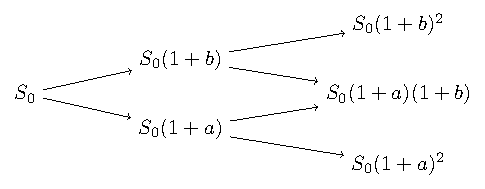
\includegraphics[width=.5\textwidth]{tikz/stochv_1_2_crr.pdf}
	\end{center}
	One also names this as a 'recombined tree model'. It has the advantage that the number of nodes grows only linearly with $n$. 
	\item Discountinious price process $\tilde{S}_n := \frac{S_n}{S_n^0} = S_0 * \prod_{k=1}^n \frac{1+R_k}{1+r}$.
	\item Filtration: natural filtration $\F_n = \sigma \brackets{S_1, \dots, S_n}$.
\end{itemize}
\begin{proposition} %2.1
	Im CRR-Modell gilt:
	\begin{enumerate}
		\item The number of upward trends $U_n := \# \set{k \in [n] \colon R_k = b}$ is binomially distributed, i.e. $U_n \sim \Bin(n,p)$.
		\item It holds
		\begin{align*}
			\log\brackets{\frac{\tilde{S}_n}{S_0}} = U_n \log\brackets{\frac{1+b}{1+a}} + n \log\brackets{\frac{1+a}{1+r}}
		\end{align*}
		d.h. $\log\brackets{\frac{\tilde{S}_n}{S_0}}$ is per Skalen-Lagen-transformation binomially distributed. 
		\item The distribution of $S_n$ is
		\begin{align*}
			\P\brackets{S_n = S_0 (1+b)^k (1+a)^{n-k}} = \binom{n}{k} p^k (1-p)^{n-k}
		\end{align*} 
	\end{enumerate}
\end{proposition}
\begin{proof}
	\begin{enumerate}
		\item clear
		\item $\frac{\tilde{S}_n}{S_0} = \brackets{\frac{1+b}{1+a}}^{U_n} * \brackets{\frac{1+a}{1+r}}^n \implies \log\brackets{\frac{\tilde{S}_n}{S_0}} = U_n \log\brackets{\frac{1+b}{1+a}} + n \log\brackets{\frac{1+a}{1+r}}$
		\item Es ist $S_n = S_0 (1+b)^{U_1}(1+a)^{n-U_n} $. Also
		\begin{align*}
			\P\brackets{S_n = S_0 (1+b)^k (1+a)^{n-k}} = \P(U_n = k) \overset{(a)}{=} \binom{n}{k} p^k (1-p)^{n-k}
		\end{align*}
	\end{enumerate}
\end{proof}
\begin{*remark}
	Part (b) suggests convergence of $\log\brackets{\frac{\tilde{S}_n}{S_0}}$ towards the normal distribution for $n \to \infty$ (per scaling) 
	$\leadsto$ Black-Scholes-Model ($\nearrow$ Chapter 3).
\end{*remark}
\begin{lemma} %2.2
	A self-financed investment strategy $(\eta_n,\xi_n)_{n\in \N}$ with initial capital $w \in \R$ and value process $\Pi_n$ are completelly defined through $w$ and $(\xi_n)_{n \in \N}$.
	\begin{itemize}
		\item The discrete value process can be represented as
		\begin{align*}
			\tilde{\Pi}_n = w + \sum_{k=1}^n \xi_k (\tilde{S}_k - \tilde{S}_{k-1}) = w + (\xi \bigcdot \tilde{S})_n
		\end{align*}
		\item The amount $\eta_n$ is uniquely given by 
		\begin{align*}
			\eta_n = \tilde{\Pi}_n - \xi_n \tilde{S}_n
		\end{align*}
	\end{itemize}
\end{lemma}
\begin{proof}
	klar!
\end{proof}
\section{Replication/Hedging of derivated in CRR-Model}
Derivative $C$ with payout $h(S_1, S_2, \dots, S_N)$ at time $N$, i.e. $C = h(S_1, S_2, \dots, S_n) \mit h$ measurable.\\
We are looking for a strategy which replicated $(\xi_n)_{n \in [N]}$ and initial capital $w$, i.e.
\begin{itemize}
	\item $(\xi_n)$ predictable with discrete value process $\tilde{\Pi}_n = w + (\xi \bigcdot \tilde{S})_n$
	\item Replication condition
	\begin{align*}
		C = h(S_1, \dots, S_N) = \Pi_N \text{   f.s. } \tag{Rep}\label{eq_2_2_rep}
	\end{align*}
\end{itemize}
\begin{definition}
	\begin{enumerate}
		\item Derivative $C$ is called \begriff{reachable}, if there exists a replication strategy.
		\item A financial model is called \begriff{complete}, if every derivative is reachable. 
	\end{enumerate}
\end{definition}
\begin{theorem} %2.3
	Let $C = h(S_1, \dots, S_N)$ be a derivative im CRR-Model. Then $C$ is reachable, i.e. $\exists w \in \R$ and $(\xi_n)_{n \in \N}$ with \eqref{eq_2_2_rep}. It holds:
	\begin{enumerate}
		\item $\exists$ measurable function $f_n \colon \R^n \to \R, n \in [N]$ so that
		\begin{align*}
			\Pi_n = f_n(S_1, \dots, S_n)
		\end{align*}
		and values of $f_n$ along the paths in the binomial tree are recursively set through
		\begin{align*}
			Rek = \begin{cases*}
				f_N(S_1, \dots, S_N) = h(S_1, \dots, S_N) = C\\
				f_n(S_1, \dots, S_N) = \frac{1}{1+r}\brackets{\frac{r-a}{b-a} f^b_{n+1} + \frac{b-r}{b-a}f^a_{n+1}} \forall n \in [N]_0
			\end{cases*}
		\end{align*}
		where $f^b_{n+1} = f_{n+1}(S_1, \dots, S_n(1+b))$ und $f^a_{n+1} = f_{n+1}(S_1, \dots, S_n(1+a))$
		\item The strategy to be replicated is given by 
		\begin{align*}
			\xi_n = \frac{f^b_n - f^a_n}{S_{n-1}(b-a)} \tag{$\Delta$-Hedge}\label{eq_2_3_hedge}
		\end{align*}
	\end{enumerate}
\end{theorem}
\begin{conclusion}
	The CRR-Model is complete.
\end{conclusion}
\begin{conclusion}
	If $C$ is an european derivative, i.e. $C = h(S_N)$, with $h\colon \R \to \R$ measurable, then the following simplifications hold: It is sufficient to take $f_n \colon \R \to \R$ and it holds
	\begin{align*}
		\Pi_n = f_n(S_n) \quad f_{n+1}^b = f_{n+1}(S_n(1+b)) \quad f^a_{n+1} = f_{n+1}(S_n(1+a))
	\end{align*}
\end{conclusion}
\begin{*remark}
	\begin{enumerate}
		\item The recursions $Rek$ corresponds to a backward iteration of the tree diagramm. Image: *tree diagram is missing :/* $f_n$ is set as discontinious mean value of $f^b_{n+1}$ and $f^a_{n+1}$. The weights $q_b = \frac{r-a}{b-a},q_a = \frac{b-r}{b-a}$. It holds: $q_a + q_b = 1$
		\item Originally the transition probabilities $p$ \emph{do not} play a role in the evaluation of $C$: it is replaced through the ``risk-neutral'' probabilities $q_b, q_a = 1-q_b$
		\item They can be efficiently implemented on the computer also for big trees
		\item The formula for $\xi_n$ is also denoted as ``Delta-Hedge''
		\begin{align*}
			\xi_n = \frac{\text{``Price reduction derivative''}}{\text{``Price reduction basic goods''}} \quad \text{difference quotient}
		\end{align*}
		\item Weitere Interpretation of $\xi_n$
		\begin{itemize}
			\item $\xi_n > 0$ The price change derivative has same sign as the price reduction basic good, there is no need of short sale!
			\item $\xi_n < 0$ Price alternation derivative has opposed sign as the price reduction basic good, there is noo need of short sale!
			\item $\xi_n \approx 0$ Price alternation derivative barely depends from the price change basic good. 
		\end{itemize}
	\end{enumerate}
\end{*remark}
\begin{proof}
	With backwards induction over  $n \in [N]_0$ 
	\begin{enumerate}
		\item For $n \in \N$ it holds: $\Pi_N = C = h(S_1, \dots, S_N)$ \eqref{eq_2_2_rep} so $\Pi_N = f_N(S_1, \dots, S_N)$ with $f_N = h$
		\item Induction step from SF-condition follows
		\begin{align*}
			&\tilde{\Pi}_{n+1} = \tilde{\Pi}_n = \xi_{n+1}(\tilde{S}_{n+1} - \tilde{S}_n) \quad | (1+r)^{n-1}\\
			&\implies \Pi_{n+1} - (1+r)\Pi_n = \xi_{n+1}(S_{n+1} - (1+r)S_n) \tag{$\ast$}\label{eq_2_4_proof}
		\end{align*}
		Per induction condition it holds $\Pi_{n+1} = f_{n+1}(S_1, \dots, S_{n+1}) = f_{n+1}(S_1, \dots, S_n, S_n (1+R_{n+1}))$ (because of the definition of CRR and $S_{n+1} = S_n(1+R_n)$).  The second cases $R_k = b$ and $R_k = a$ can occur respectively with strictly positive probability. 
		\begin{itemize}
			\item[Case 1:] $\Pi_{n+1} = F_{n+1}(S_1, \dots, S_n, S_n(1+b)) = f^b_{n+1}$, substitution in \eqref{eq_2_4_proof}, yields
			\begin{align*}
				f^b_{n+1} - (1+r)\Pi_n = \xi_{n+1}S_n(b-r) \tag{I}\label{eq_2_4_I}
			\end{align*}
			\item[Case 2:] $S_{n+1} = S_n(1-a)$ und $\Pi_{n+1} = f_{n+1}(S_1, \dots, S_n, S_n(1+a)) = f^a_{n+1}$, substitution in \eqref{eq_2_4_proof}, yields
			\begin{align*}
				f^a_{n+1} - (1+r)\Pi_n = \xi_{n+1}S_n(a-r) \tag{II}\label{eq_2_4_II}
			\end{align*}
		\end{itemize}
		$\Pi_n$ is $\xi_{n+1}$ $\F_n$-measurable, meaning independent from $R_{n-1} \implies$ \eqref{eq_2_4_II} \eqref{eq_2_4_I}
		\begin{itemize}
			\item \eqref{eq_2_4_II} - \eqref{eq_2_4_I}: $f^b_{n+1} - f^a_{n+1} = \xi_{n+1} S_n(b-a)$, then $\xi_{n+1} = \frac{f^b_{n+1} - f^a_{n+1}}{S_n(b-a)}$ so \eqref{eq_2_3_hedge} \checkmark
			\item in \eqref{eq_2_4_I} $f^b_{n+1}-(1+r)\Pi_n = \frac{b-r}{b-a}(f^b_{n+1}-f^a_{n+1})$, then $\Pi_n = \frac{1}{1+r} \brackets{\frac{r-a}{b-r}f^a_{n+1} + \frac{b-r}{b-a}f^a_{n+1}} \implies \eqref{eq_2_2_rep}$ \checkmark
		\end{itemize}
	\end{enumerate}
\end{proof}
\begin{*remark}
	Systems of linear equations  \eqref{eq_2_4_I} + \eqref{eq_2_4_II} can be written as
	\begin{align*}
		\begin{pmatrix}
			1+r & b-r \\
			1+r & a-r
		\end{pmatrix} 
		\begin{pmatrix}
			\Pi_n\\
			\xi_{n+1} S_n
		\end{pmatrix} = 
		\begin{pmatrix}
			f^b_{n+1}\\
			f^a_{n+1}
		\end{pmatrix} \tag{SLE-1}\label{eq_LGS_1}
	\end{align*}
\end{*remark}
\begin{*example}
	``Asiatic call-option'', payout:
	\begin{align*}
		C=(\overline{S}_N - K)_+ \mit \overline{S}_N = \frac{1}{1+N}\sum_{k=0}^N S_k
	\end{align*}
	Path dependent derivative. Evaluation in CRR-model with $N=2$ with parameter:
	\begin{align*}
		b=0,3\quad a=0,3 \quad r = 0,2\quad S_0 = 100\quad K = 100
	\end{align*}
	Binomial tree:
	\begin{center}
		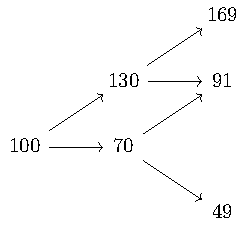
\includegraphics[width=.5\textwidth]{tikz/stochv_2_3.pdf}
	\end{center}
	\begin{align*}
		C&=h(S_1,S_2) \mit h = f_2\\
		h(130,169) &= (\frac{399}{3}-100)_+ = 33\\
		h(130,91) &= (\frac{321}{3}-100)_+ = 7\\
		h(70,91) &= (\frac{261}{3}-100)_+ = 0\\
		h(70,49) &= (\frac{219}{3}-100)_+ = 0
	\end{align*}
	Recursion:\\
	\begin{align*}
		\text{Auxiliary calculation: }q = \frac{r-a}{b-a} &= \frac{0,4}{0,6} = 2/3 \und 1-a = 1/3\\
		f_1(130) &= \frac{1}{1+r}(q \cdot f^b + (1-q)f^a)\\
		&= \frac{1}{1,1}(2/3 33 + 1/3 7) = \frac{1}{1,1}\cdot 73/3\\
		&\approx 22,12\\
		f_1(70) &= \frac{1}{1,1}(2/3 0 + 1/3 0) = 0\\
		f_0 &= \frac{1}{1,1}(2/3 \frac{1}{1,1} 73/3 + 1/\cdot 0) \approx 13,41
	\end{align*}
	Strategy:
	\begin{align*}
		\xi_2(130) &= \frac{f_2^b - f_2^a}{S_1 (b-a)} = \frac{33-7}{130\cdot 0,6} = \frac{26}{13\cdot 6} = 1/3\\
		\xi_2(70) &= \frac{0-0}{70\cdot 0,6} = 0\\
		\xi_1 &= \frac{f_1^b - f_1^a}{S_0(b-a)} = \frac{\frac{1}{1,1}73/3 - 0}{100\cdot 0,6} = \frac{73}{3\cdot 11 \cdot 6} = \frac{73}{196} \approx 0,37 
	\end{align*}
\end{*example}
\section{Martingale and arbitrage in CRR-model}
Consider a CRR-model on a probability space $(\O,\F,\P)$. Set another probability measure $\QQ$ on $(\O,\F)$. I.e. we leave the structure of the tree unaltered, but we change the transition probability:
\begin{align*}
	\text{ von }p = \P(R_n = b)\\
	\text{ zu }q = \QQ(R_n = b)
\end{align*}
Notation: $\E^{\QQ}[\cdot]$ expected value under $\QQ$.
\begin{definition}
	A probability measure $\QQ$ on $(\O,\F)$ is called equivalent martingale measure (EMM) for the CRR-model, if it holds
	\begin{enumerate}
		\item $\QQ\sim \P$ ($\QQ$ equivalent to $\P$)
		\item discrete price process $(\tilde{S}_n)_{n \in [N]}$ is $\QQ$-martingale, i.e.
		\begin{align*}
			\E^{\QQ}[\tilde{S}_{n+1}\mid \F_n] = \tilde{S}_n \quad \forall n \in [N-1]_0
		\end{align*}
	\end{enumerate}
\end{definition}
\begin{erinnerung}
	$\P, \QQ$ probability measures on $(\O,\F)$
	\begin{itemize}
		\item $\P \sim \QQ :\Leftrightarrow (\P(A) = 0 \Leftrightarrow \QQ(A) = 0 \forall A \in \F$ (equivalent)
		\item $\QQ << \P \Leftrightarrow (\P(A) = 0 \implies \QQ(A) = 0 \forall A \in \F$ ($\QQ$ absolute continious with respect to $\P$)
		\item It holds: $\QQ \sim \P \Leftrightarrow (\QQ << \P \wedge \P << \QQ)$
	\end{itemize}
\end{erinnerung}
\begin{theorem}
	\begin{enumerate}
		\item In CRR-model there exists a EMM iff it holds $a < r < b$
		\item The EMM $\QQ$ is unique and it holds
		\begin{align*}
			q &:= \QQ(R_n = b) = \frac{r-a}{b-a}\\
			1-q &= \QQ(R_n = a) = \frac{b-r}{b-a} \quad \forall n \in [N]
		\end{align*}
	\end{enumerate}
\end{theorem}
\begin{*remark}
	$q$ and $1-q$ are exactly the risk-neutral weights, which appear in \eqref{eq_2_2_rep}
\end{*remark}
\begin{proof}
	Let $\QQ$ be an arbitrary probability measure on $(\O,\F)$. Set
	\begin{align*}
		q_n &:= \Q(R_n = b\mid \F_{n-1}) \in [0,1]\\
		\E^{\QQ}[\tilde{S}_n \mid \F_{n-1}] &= \E^{\QQ}[\tilde{S}_n \cdot (\frac{1+R_n}{1+r}) \mid \F_{n-1}]\\
		&= \tilde{S}_{n-1}\frac{1}{1+r}\E^{\QQ}[1+R_n \mid \F_{n-1}]\\
		&= \tilde{S}_{n-1} \cdot \frac{1}{1+r}(q_n(1+b) + (1-q_n)(1+a))
		\intertext{Then}
		(\tilde{S}_{n \in[N]}) \text{ ist $\QQ$-martingale} \Leftrightarrow\\
		\frac{1}{1+r}(q_n (1+b) + (1-q_n)(1-a) = 1 \quad \forall n\\
		q_n b = (1-q_n)a = r\\
		q_n (b-a) = r-a \implies q_n = \frac{r-a}{b-a}
	\end{align*}
	\begin{align*}
		q_n \in[0,1] \Leftrightarrow a \le r \le b\\
		\QQ \sim \P\colon q_n \in (0,1) \Leftrightarrow a < r < b
	\end{align*}
	i.e. $\QQ$ is EMM $\Leftrightarrow a < r < b$.
\end{proof}
\begin{theorem}[Risk-neutral evaluation formula]
	Let $C = h(S_1, \dots, S_n)$ be a derivative in CRR-model with EMM $\QQ$. For the price process $(\Pi_n)_{n \in [N]}$ of $C$ it holds:
	\begin{align*}
		\Pi_n = (1+r)^{-(N-n)}\cdot \E^{\QQ}[C \mid \F_n]
		\intertext{It especially holds}
		w = \Pi_0 = (1+r)^{-N} \cdot \E^{\QQ}[C]
	\end{align*}
	\emph{In words:} The fair price of $C$ is unique and given by the discontinious expected value of $C$ \emph{under the martingale measure $\QQ$}.
\end{theorem}
\begin{proof}
	The probability space for the CRR-model is finite, i.e. $\abs{\O} = 2^N < \infty$ (finitely many paths in CRR-model). Hence, every random variable is bounded and especially $C$ and $(\xi_n)_{n \in [N]}$. Let $(\xi_n)$ be a replication strategy for $C$ with discontinious value process $(\tilde{\Pi}_n)$, i.e. 
	\begin{align*}
		\tilde{\Pi}_n = w + \sum_{k=1}^n \xi_k (\tilde{S}_k - \tilde{S}_{k-1}) = w+ (\xi \bigcdot \tilde{S})_n
		\intertext{und}
		\tilde{\Pi}_n = (1+r)^{-N}C
	\end{align*}
	$\QQ$ is EMM $\implies (\tilde{S}_n)$ is $\QQ$-martingale. With Theorem 1.6 $(\xi \bigcdot \tilde{S})_n$ is $\QQ$-martingale. Hence it follows $\tilde{\Pi}_n$ is $\QQ$-martingale.
	\begin{align*}
		\Pi_n &= (1+r)^n \cdot \tilde{\Pi}_n = (1+r)^n \E^{\QQ}[\Pi_N \mid \F_n] \quad \text{martingale}\\
		&= (1+r)^{-(N-n)} \cdot \E^{\QQ}[C \mid \F_n].
	\end{align*}
\end{proof}
\begin{*remark}[to martingale condition for $\QQ$]
	We write (somewhat incovenietly)
	\begin{itemize}
		\item $q_b = \QQ(R_n = b)$ und $q_a = \QQ(R_n = a)$
		\item $\QQ$-measure: $q_a + q_b = 1 \Leftrightarrow q_b(1+r) + q_a (1+r) = 1+r$
		\item Martingale condition:
		\begin{align*}
			(1+b)q_b + (1+a)q_a = 1-r \Leftrightarrow q_b(b-r) + q_a(a-r) = 0
		\end{align*}
		As a system of linear equations:
		\begin{align*}
			\begin{pmatrix}
				1+r & 1+r \\
				b-r & a-r
			\end{pmatrix}
			\begin{pmatrix}
				q_b\\ q_a
			\end{pmatrix} =
			\begin{pmatrix}
				1+r\\ 0
			\end{pmatrix} \tag{SLE-2}\label{eq_2_4_LGS2}
		\end{align*}
		is a condition for martingale measure. Compare with 
		\begin{align*}
			\begin{pmatrix}
				1+r & 1+r \\
				b-r & a-r
			\end{pmatrix}
			\begin{pmatrix}
				\Pi_{n+1}\\ \xi_n \cdot S_{n-1}
			\end{pmatrix} =
			\begin{pmatrix}
				f_n^b\\ f_n^a
			\end{pmatrix}
		\end{align*}
		the latter is again \eqref{eq_LGS_1}, the same matrix but transposed $\implies$ \begriff{duality}!
	\end{itemize}  
\end{*remark}
\subsection*{Arbitrage in CRR-model}
\begin{definition}
	An investment strategy $(\xi_n)_{n \in[N]}$ with time horizon $N$ and discontinious value process $(\tilde{\Pi}_n)_{n \in [N]}$ is called \begriff{an arbitrage}, if it holds:
	\begin{enumerate}
		\item $\tilde{\Pi}_0 = 0$ (no initial capital)
		\item $\P(\tilde{\Pi}_N \ge 0) = 1$ (no risk of loss)
		\item $\P(\tilde{\Pi}_N > 0) > 0$ (positive profit with positive probability)
	\end{enumerate}
	We negotiate the 3 conditions (arb.) % find a way to reference to all 3 :(
\end{definition}
\begin{theorem} %2.8
	In CRR-model are equivalent
	\begin{enumerate}
		\item There does not exist an arbitrage (NA = ``No-arbitrage'')
		\item There exists an EMM $\QQ$ 
	\end{enumerate}
\end{theorem}
\begin{*remark}
	This Theorem basically holds in \emph{all} financial models (discrete, continious, ...). It is also called \emph{1. Main theorem of the price theory}.
\end{*remark}
\begin{proof}
	\begin{itemize}
		\item b)$ \implies$ a) with contradiction. Let $\QQ$ be an EMM \emph{and} $(\xi)$ arbitrage. Because of $\QQ \sim \P$ it follows from (arb):
		\begin{align*}
			\QQ(\tilde{\Pi}_N \ge 0) = 1\\
			\QQ(\tilde{\Pi}_N > 0) > 0\\
			\implies \E^{\QQ}[\tilde{\Pi}_N] > 0 \tag{$\ast$}\label{eq_2_4_2_8}
		\end{align*}
		Otherwise: $\tilde{\Pi}_N = 0 + (\xi \bigcdot \tilde{S})_N$. $\tilde{S}$ is $\QQ$-martingale $\implies (\xi \bigcdot \tilde{S})$ is $\QQ$-martingale, then
		\begin{align*}
			\E^{\QQ}[\tilde{\Pi}_N] = \E^{\QQ}((\xi \bigcdot \tilde{S})_N) = 0
		\end{align*}
		and that is a contradiction to \eqref{eq_2_4_2_8}.
	\end{itemize}
\end{proof}